\documentclass[varwidth=true,border=2pt]{standalone}
\usepackage{circuitikz}

\begin{document}
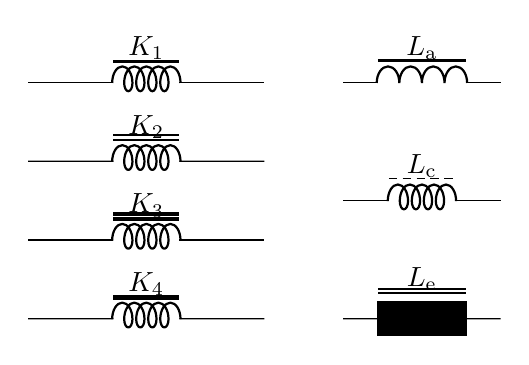
\begin{tikzpicture}[american]
  % Adapted from the TeX Live circuitikz manual's choke and core-anchor examples.
  \draw (0,0) to[cute choke, name=K1, l=$K_1$] ++(3,0);
  \draw (0,-1) to[cute choke, twolineschoke, name=K2, l=$K_2$] ++(3,0);
  \ctikzset{bipoles/cutechoke/cthick=2, twolineschoke}
  \draw (0,-2) to[cute choke, name=K3, l=$K_3$] ++(3,0);
  \draw (0,-3) to[cute choke, onelinechoke, name=K4, l=$K_4$] ++(3,0);

  \ctikzset{american}
  \draw (4,0) to[L, l=$L_{\mathrm{a}}$, name=A] ++(2,0);
  \draw[thick] (A.core west) -- (A.core east);
  \ctikzset{cute inductors}
  \draw (4,-1.5) to[L, l=$L_{\mathrm{c}}$, name=C] ++(2,0);
  \draw[densely dashed] (C.core west) -- (C.core east);
  \ctikzset{european, bipoles/inductors/core distance=4pt}
  \draw (4,-3) to[L, l=$L_{\mathrm{e}}$, name=E, label distance=2pt] ++(2,0);
  \draw[thick, double] (E.core west) -- (E.core east);
\end{tikzpicture}
\end{document}
